\documentclass[aspectratio=169]{beamer}
\usepackage{xeCJK}
\setCJKmainfont{OPPO Sans}

\usepackage{Handle}

\newcommand{\Title}{标题}
\newcommand{\Subtitle}{副标题}
\newcommand{\Institute}{机构名称}
\newcommand{\InstituteAddress}{机构地址}
\newcommand{\SubmittedBy}{提交人}
\newcommand{\SubmittedTo}{提交给}
\newcommand{\ImageUrl}{Images/graph.jpg}

\subject{DAA}

\small
\date{\today}

\begin{document}
\section{图的类型}

	\setbeamercolor{section in head/foot}{bg=cyan,fg=black}
	\setbeamercolor{frametitle}{bg=aqua,fg=black}
	\setbeamercolor{author in head/foot}{bg=aqua,fg=black}

	\begin{frame}[t,allowframebreaks]{图的类型}
  \vspace{-5mm}
		\begin{bee}[完全图,width = 8cm]{white}{deepmagenta}
			一个图,其中每一对不同的节点都通过一条边相连
		\end{bee}
           \vspace{-5mm}
		\begin{Rbee}[森林,width = 0.86\paperwidth]{white}{arsenic}
			图中一组树或不相交的树状结构
		\end{Rbee}
   % \vspace{-5mm}
		\begin{bee}[树,width = 0.9\paperwidth]{white}{blue}
			一个特殊的无环图,其中有一个根节点,其他每个节点都通过一条边与根节点相连。
		\end{bee}
\begin{columns}
			\column{0.5\textwidth}
			\begin{bee}[无向图,width = 6cm]{black}{aqua}
				一个图,其中边没有方向。
			\end{bee}
			\column{0.55\textwidth}
			\begin{Rbee}[有向图,width = 6cm]{arsenic}{aqua}
				一个图,其中边有方向。
			\end{Rbee}
		\end{columns}
		\begin{figure}
			\centering
			\href{https://media.geeksforgeeks.org/wp-content/uploads/20200630114438/directed.jpg}{
				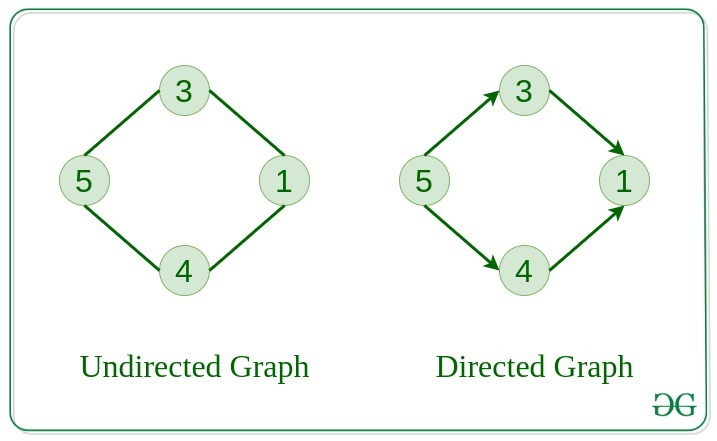
\includegraphics[height =0.37\paperheight]{Images/directed.png}
			}
		\end{figure}
	\end{frame}

	\begin{frame}[noframenumbering,plain,t]

		\begin{tikzpicture}[remember picture, overlay]
			\node[opacity = 0.8] at (current page.center)
			{
				
\includegraphics[height = 1.5\paperwidth]{Images/bg4.png}
			};
		\end{tikzpicture}

		\MakeTitle

	\end{frame}


	\begin{frame}{大纲}
		\begin{tikzpicture}[remember picture, overlay]
			\node[opacity = 0.2] at (current page.center)
			{
				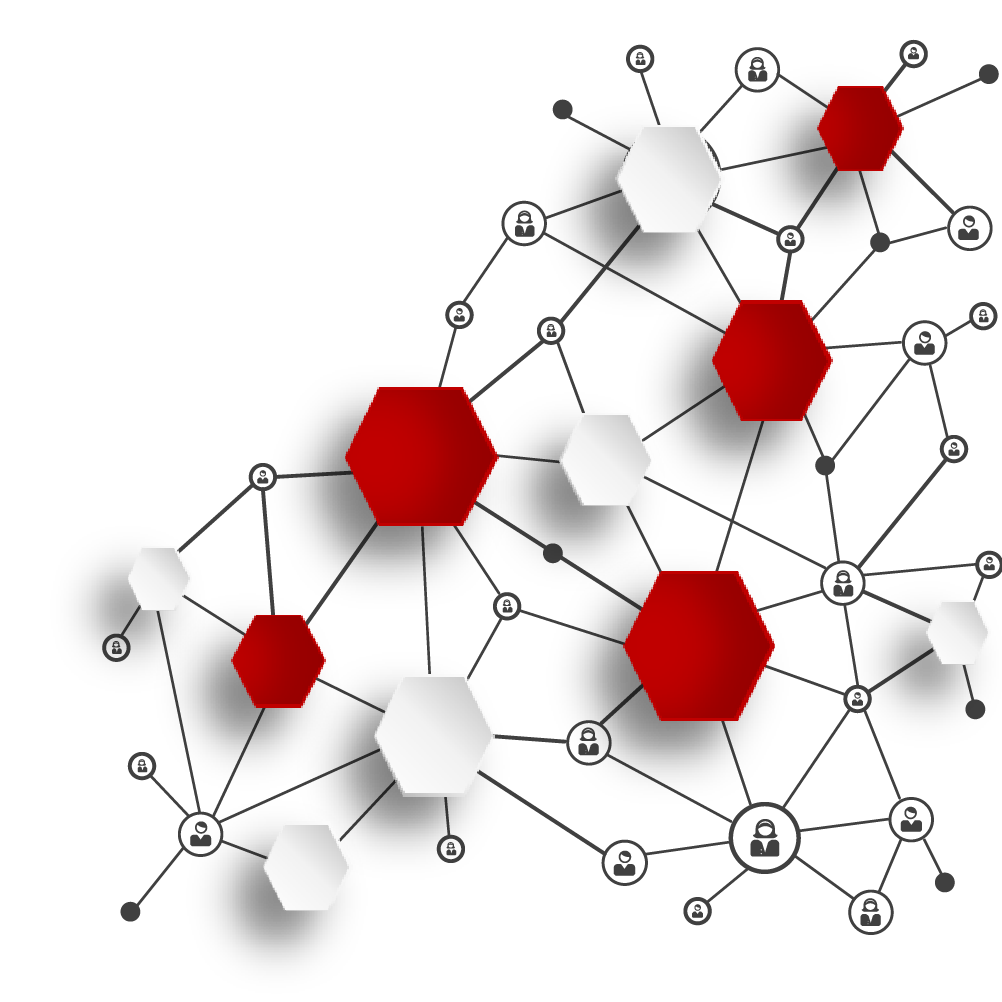
\includegraphics[height = 0.75\paperwidth]{Images/bg3.png}
			};
		\end{tikzpicture}

		\normalsize
		\tableofcontents
	\end{frame}


	\section{介绍}
	   \setbeamercolor{section in head/foot}{bg=arsenic,fg=white}
	\setbeamercolor{frametitle}{bg=airforceblue,fg=white}
	\setbeamercolor{author in head/foot}{bg=arsenic,fg=white}

	\begin{frame}[t,allowframebreaks]{图的介绍}

		\begin{itemize}
			\item  图是一种由顶点和边组成的非线性数据结构。
			\item \textbf{顶点}有时也称为节点,而\textbf{边}是连接图中任意两个节点的线或弧。

			\begin{bee}[更正式地]{white}{arsenic}
				图由一组顶点V和一组边E组成。 \\
				图用\textbf{G(V,E)}表示。
			\end{bee}

			\item 图数据结构是表示和分析对象或实体之间复杂关系的强大工具。
			\item 它们在社交网络分析、推荐系统和计算机网络等领域特别有用。
			\item 在体育数据科学领域,图数据结构可以用来分析和理解团队表现和球员在场上互动的动态。

		\end{itemize}

	\end{frame}

	
\end{document}